\section{Method}
\label{sec:method}

Our method, \textbf{ResponseVec}, comprises four stages: (i) construction of a literature-grounded survey prompt that fuses the demographic profile, target-relevant answer history, and the current item with its full option set; (ii) extraction of a latent reaction vector via a generative LLM embedder; (iii) prediction by an option-aware, calibratable decoder; and (iv) a reusable RespondentVec variant that amortizes compute across items. Figure~\ref{fig:framework} summarizes the pipeline. We detail each stage and then formalize the option-aware decoder, which is the principal methodological contribution.

\begin{figure}[tb]
\centering
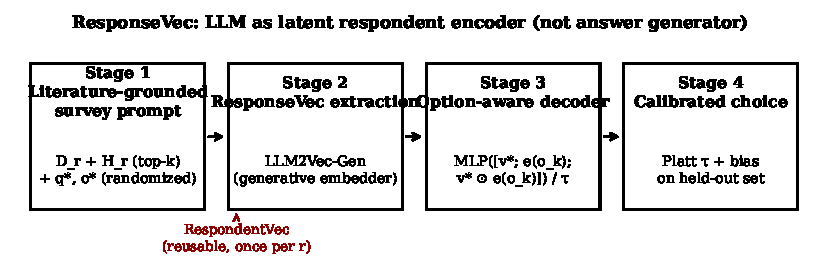
\includegraphics[width=\columnwidth]{figures/figure1_framework.pdf}
\caption{The ResponseVec pipeline. The LLM is repurposed from answer generator (dashed off-path token) to latent respondent encoder. Stages 1--3 form the query-conditioned ResponseVec; the RespondentVec branch encodes the respondent once and reuses the vector across items.}
\label{fig:framework}
\end{figure}

\subsection{Literature-Grounded Survey Prompt}
\label{sec:prompt}

For a target item $(r,q^\ast,o^\ast)$, we construct a prompt $P(r,q^\ast)$ from three sources. The \emph{demographic block} $D_r$ is rendered as a structured template following established survey-administration conventions (e.g., ISSP respondent-profile wording), which avoids position and framing biases documented in prior silicon-sampling work~\citep{hu2024quantifying,venkit2026need}. The \emph{history block} retrieves the top-$k$ prior records from $H_r$ most relevant to $q^\ast$, where relevance is computed as cosine similarity between the LLM2Vec-Gen embedding of $q^\ast$ and that of each prior question $q_i$; critically, each retrieved record retains the full option set $o_i$ and the chosen answer $a_i$, so the model is conditioned on the respondent's revealed preferences over concrete alternatives rather than on free-text summaries. The \emph{item block} presents the question stem $q^\ast$ together with the full option set $o^\ast$, with option order randomized per call to suppress position bias. This ``literature-grounded'' construction ensures the prompt mirrors the actual administration of a survey instrument rather than an informal paraphrase, which prior work has shown is essential for faithful respondent simulation~\citep{su2026adaptive,li2026personabased}.

\subsection{Latent Reaction Vector Extraction}
\label{sec:extraction}

We extract the ResponseVec using LLM2Vec-Gen~\citep{behnamghader2026llmvecgen}, a self-supervised generative embedding method that maps a decoder-only LLM to an encoder while preserving the model's output distribution semantics. Formally, given the prompt $P(r,q^\ast)$, the ResponseVec is
\begin{equation}
\mathbf{v}^\ast_r = g_\theta(P(r,q^\ast)) \in \mathbb{R}^d,
\end{equation}
where $g_\theta$ denotes the LLM2Vec-Gen encoder. We aggregate representations across multiple transformer layers via a learnable layer-weighting $\sum_{\ell} \alpha_\ell \, \mathbf{h}^{(\ell)}$ rather than relying on the last layer alone, since lower layers carry item-level lexical structure that complements the higher layers' semantic abstractions. Two design choices distinguish $\mathbf{v}^\ast_r$ from alternatives. First, against raw hidden states, LLM2Vec-Gen applies bidirectional attention and contrastive alignment, producing an isotropic, choice-aligned geometry that supports downstream calibration. Second, against a discriminative encoder such as LLM2Vec~\citep{behnamghader2024llmvec}, LLM2Vec-Gen's generative training objective retains the LLM's output semantics, so $\mathbf{v}^\ast_r$ encodes a latent disposition to \emph{generate} particular answers rather than a retrieval-optimized representation detached from generation. We optionally continue the contrastive training of $g_\theta$ on a small auxiliary corpus of survey question--answer pairs to sensitize the representation to the item--option structure, though our main results use the off-the-shelf encoder.

\subsection{Option-Aware Decoder}
\label{sec:decoder}

The decoder $h_\phi$ is the component that anchors the latent reaction vector to the concrete option distribution of the target instrument and renders the system calibratable. We detail its construction, which is the principal methodological contribution of this work.

\paragraph{Option embeddings.} Each option text $o_k$ is encoded by the same generative embedder $g_\theta$ used for the prompt, yielding an option embedding $\mathbf{e}(o_k) = g_\theta(o_k) \in \mathbb{R}^d$. Using the same encoder ensures that $\mathbf{v}^\ast_r$ and $\mathbf{e}(o_k)$ live in a shared semantic space, so their interaction is meaningful. We additionally encode the question stem to obtain $\mathbf{e}(q^\ast)$, which is used only in the reusable RespondentVec regime (Section~\ref{sec:respondentvec}).

\paragraph{Scoring function.} For the query-conditioned ResponseVec $\mathbf{v}^\ast_r$, the score for option $k$ is
\begin{equation}
\label{eq:score}
s_k = \mathrm{MLP}_\phi\!\left( \left[\, \mathbf{v}^\ast_r \,;\, \mathbf{e}(o_k) \,;\, \mathbf{v}^\ast_r \odot \mathbf{e}(o_k) \,\right] \right),
\end{equation}
where $[\,;\,]$ denotes concatenation and $\odot$ the elementwise product. The concatenation supplies the decoder with both the independent terms and their multiplicative interaction, the latter capturing the extent to which the respondent's latent reaction aligns with the option's semantic content. The predicted choice distribution is
\begin{equation}
\label{eq:softmax}
\hat{p}(y^\ast = k \mid r, q^\ast) = \frac{\exp(s_k / \tau)}{\sum_{j=1}^{K} \exp(s_j / \tau)},
\end{equation}
where $\tau > 0$ is a learnable temperature. The decoder $\mathrm{MLP}_\phi$ is intentionally tiny---two hidden layers of width 128 with ReLU activations, totaling fewer than $10^5$ parameters---so that it cannot memorize respondent--item pairs and must instead learn a generalizable mapping from reaction--option interaction to choice.

\paragraph{Calibration.} The temperature $\tau$ and a per-option bias vector $\mathbf{b} \in \mathbb{R}^K$ are fit on a small held-out calibration set by minimizing the negative log-likelihood, which is equivalent to Platt scaling generalized to the multinomial case~\citep{filho2023classifier}. Because the decoder is so small, this calibration step is computationally trivial and can be performed per-instrument, yielding a system whose predicted probabilities are faithful to the empirical choice distribution of the target survey. We additionally consider a sample-dependent temperature variant $\tau(\mathbf{v}^\ast_r)$ following \citet{joy2023sampledependent}, in which a small head regresses the temperature from the reaction vector, allowing high-confidence and low-confidence respondents to be sharpened or softened differently.

\paragraph{Why option-awareness matters.} A decoder that scores options independently of their text---for instance, a linear head mapping $\mathbf{v}^\ast_r$ directly to a $K$-way logits vector---is forced to relearn the option semantics from scratch and cannot transfer across instruments whose option sets differ. By making the decoder a function of the option embeddings, we decouple the representation of the respondent's reaction ($\mathbf{v}^\ast_r$) from the representation of the instrument's options ($\mathbf{e}(o_k)$), so that the same decoder transfers across questionnaires with different option sets, different numbers of options, and different option wordings. This is the survey-domain analogue of the city-agnostic downstream model in \citet{he2025geolocation}, and it is what enables the cross-instrument and cross-wave transfer we report in Section~\ref{sec:results}.

\subsection{Reusable RespondentVec}
\label{sec:respondentvec}

The query-conditioned ResponseVec requires a fresh LLM forward pass for every target item, which is costly when an entire questionnaire is to be imputed for a respondent. We therefore define a reusable variant,
\begin{equation}
\mathbf{v}_r = g_\theta(P(D_r, H_r)),
\end{equation}
which encodes only the demographic profile and the answer history, omitting the target item. The target item enters at the decoder:
\begin{equation}
\label{eq:score_reuse}
s_k = \mathrm{MLP}_\phi\!\left( \left[\, \mathbf{v}_r \,;\, \mathbf{e}(q^\ast) \,;\, \mathbf{e}(o_k) \,;\, \mathbf{v}_r \odot \mathbf{e}(q^\ast) \,;\, \mathbf{v}_r \odot \mathbf{e}(o_k) \,\right] \right).
\end{equation}
Here $\mathbf{v}_r$ is computed once per respondent and reused across all $q^\ast$, so the per-item cost reduces to a single forward pass through the tiny decoder rather than through the LLM. The trade-off is that $\mathbf{v}_r$ cannot encode item-specific reaction; it encodes only a stable respondent disposition, and the decoder must infer the item-specific reaction from the interaction of $\mathbf{v}_r$ with $\mathbf{e}(q^\ast)$ and $\mathbf{e}(o_k)$. Section~\ref{sec:tradeoff} formalizes when this loss of query conditioning is acceptable.

\subsection{Training and Inference}
\label{sec:training}

The decoder parameters $\phi$ (MLP weights, temperature, biases) are trained on the survey training split by minimizing the cross-entropy between $\hat{p}$ and the true choice $y$, with $\ell_2$ regularization on $\phi$ and early stopping on a validation split. The encoder $g_\theta$ is frozen in our main experiments; the optional continued-contrastive variant fine-tunes $g_\theta$ on survey question--answer pairs with a contrastive objective before freezing. At inference, the per-respondent cost is one LLM forward pass (RespondentVec) plus $K$ decoder forward passes, or $Q$ LLM forward passes (ResponseVec) for a questionnaire of $Q$ items. The decoder cost is negligible, so the ResponseVec/RespondentVec cost ratio scales as $\Theta(Q)$ per respondent, which we exploit in the cost analysis of Section~\ref{sec:tradeoff}.
